%% Chapter 2
%% NOTES: :set tw=79 to set the text width and also make sure 
%%        :set formatoptions+=t
\chapter{Top-Down Inversion Framework}

 \section{Introduction}
 After emiting into atmosphere, aerosol particles undergo various 
processes including turbulent mixing, chemistry, convection, and tranport
before removed from the atmosphere via dry and wet depositions. Satellite
measurements, like AOD, provide indeed a snapshot of the aerosol distribution
in the atmosphere. Therefore, Contraining aerosol emissions from satellite
remote sensing observations involves two types of development, i.e., the
forward modeling and inverse modeling. Mathematically, the forward modeling
constructs a complete a physical system to predict the outcome of measurements. 
The inverse modeling uses the actual measurements to infer the values of the
parameters that characterize the system. Particularly for this work (Figure
\ref{fig:td_flow}), we use the GEOS-Chem chemistry transport model as the
forward operator to simulate the relevant satellite measurements. The GEOS-Chem
adjoint model is used to seek the improved aerosol emission estimates and dust
source parameterization from these measurements.

In the following sections of this chapter, I first briefly present the
inverse problem theories (\ref{sec:inv}),
then describe the GEOS-Chem chemistry transport model that acts as forward 
operator (model) in the inversion framework (\ref{sec:gc}), and finally
introduce the developement of the adjoit of GEOS-Chem model (\ref{sec:gcadj}).

 \begin{figure}[t]
  \centering
  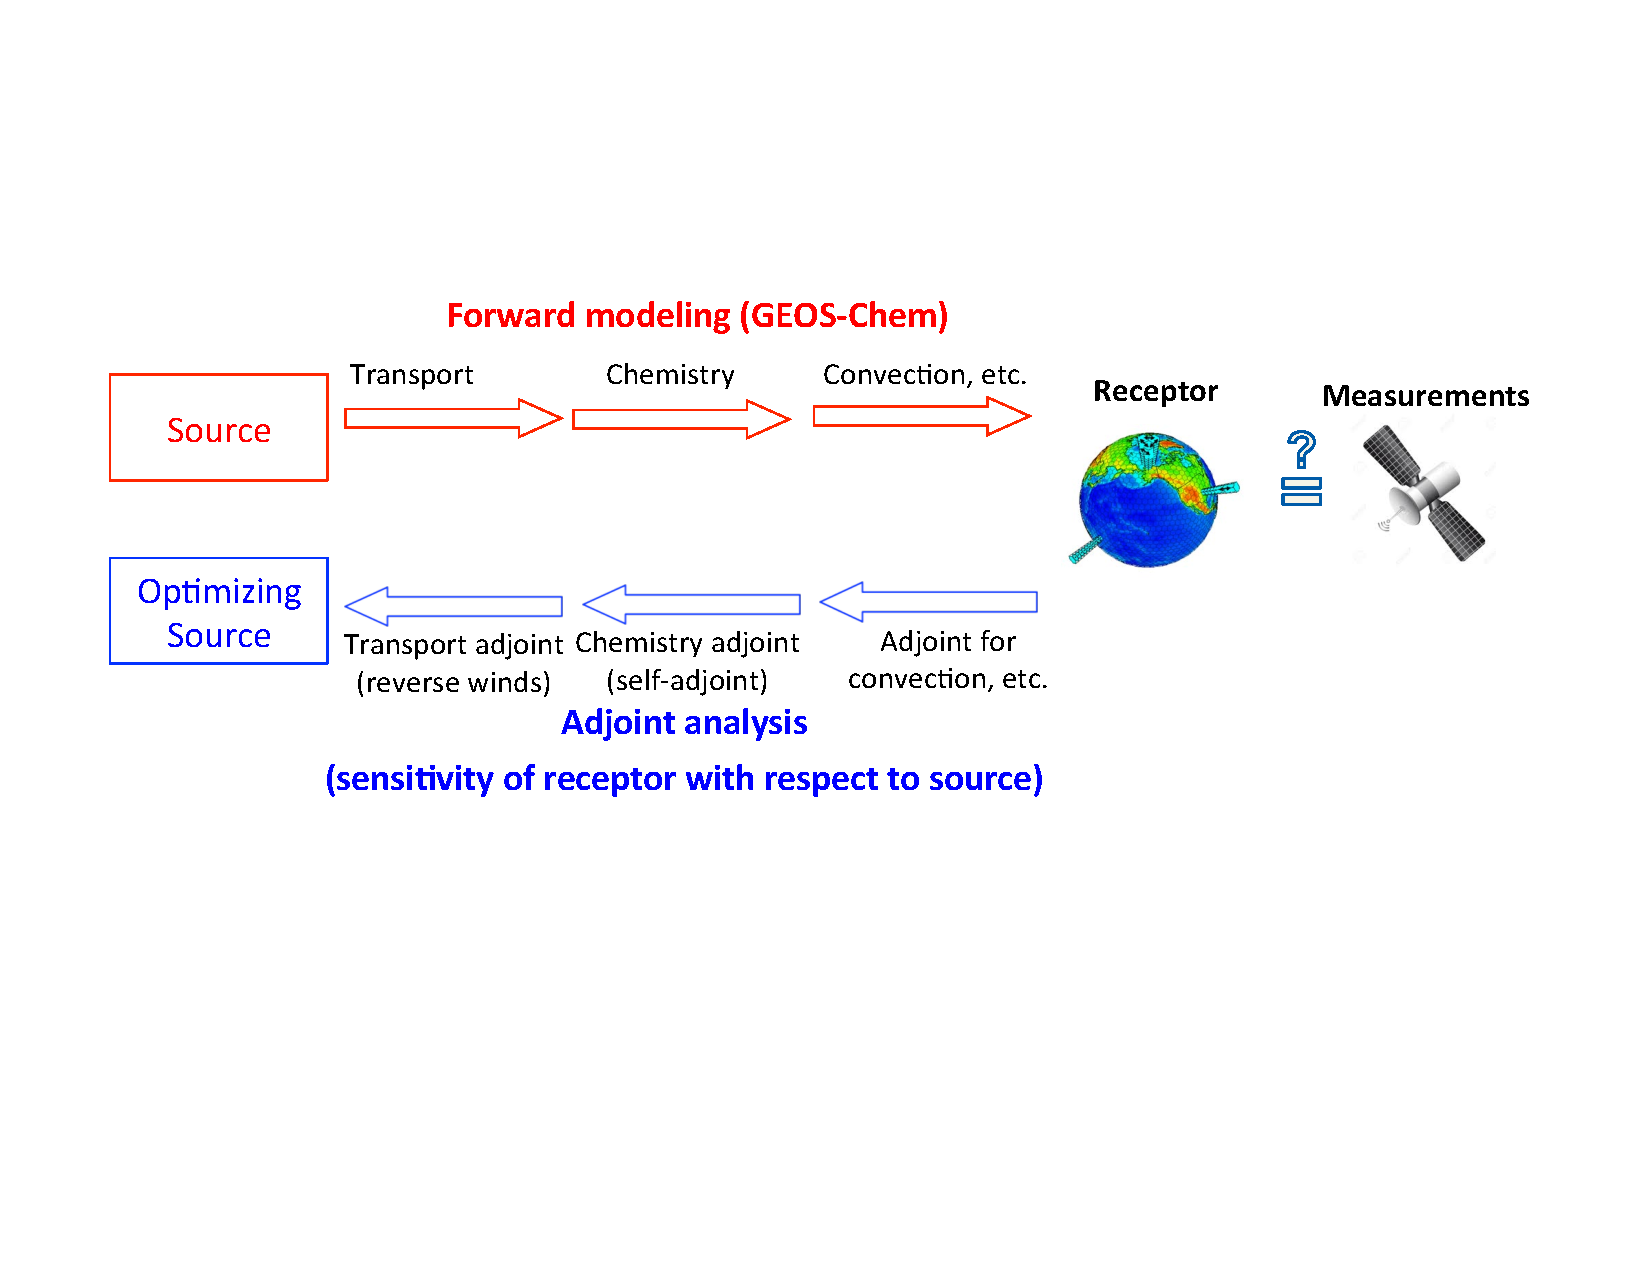
\includegraphics[width={\textwidth}]{figures/201.pdf}
  \caption{Flowchart of the proposed top-down inversion framework}
  \label{fig:td_flow}
 \end{figure}

\section{Inverse Problem Theory} \label{sec:inv}

Let $\mathbf{x}$ denote a state vector of $n$ parameters to be constrained
 and $\mathbf{y}$ an observation vector assembled by $m$ measurements,
 and let $\mathbf{F}$ indicate a forward model that describes the physics of
 the measurement process. Then, we can express the relationship between
 the observation vector and the state vector as
 \begin{equation} \label{eq:fx}
 \mathbf{y} = \mathbf{F}(\mathbf{x}) + \bdeps \mbox{,}
 \end{equation}
 where $\bdeps$ is an experimental error term that includes
 observation noise and forward modeling uncertainty.

 For this work, the observation
 vector $\mathbf{y}$ comprises measurements of
 aerosol loading, such as mass concentrations or optical depth, at any temporal
 and spatial scale. The components of the sate vector $\mathbf{x}$ could vary
 according to our inversion focus. For the inversion of aerosol emission estimats
 (as in the Chapter \ref{chap:optems}),
 $\mathbf{x}$ comprises the emission fluxes (or their scaling factors) of defined
 aerosol species within each grid cell of specified temporal resolution.
 In constrast, $\mathbf{x}$ consists of
 dust emitting parameters (or their scaling factors) when we tend to constrain
 the dust emission parameterization (as in the Chapter \ref{chap:optdead}).
 The forward model $\mathbf{F}$
 represents the GEOS-Chem that maps parameters from the state space to the
 observation space. The inversion of the state vector from these measurements is often
 an ill-posed problem due to non-linearity and limited sensitivity of these observed
 quantities to the constrained parameters. We need to combine additional constraints
 to make the problem amenable to inversion.

 \textit{A propri} information describes our knowledge of the state vector before measurements
 are applied. \textit{A propri} constraint is commonly used to achieve a well-defined stable
 and physically reasonable solution to an ill-posed problem. Usually, \textit{a propri}
 knowledge comprises both a mean state $\bdxa$ and its error
 $\bdeps_\text{a}$:
 \begin{equation} \label{eq:xa}
  \mathbf{x} = \bdxa + \bdeps_\text{a}
 \end{equation}

 Under assumption of Gaussian-distributed errors, the Maximum A Posteriori solution of
  equations \eqref{eq:fx} and \eqref{eq:xa} according to the Bayesian approach
 corresponds to the state vector that minimizes the quadratic cost function
 \citep{rodgers00}:
 \begin{equation} \label{eq:cost}
 J(\mathbf{x}) = \frac{1}{2} \left[ \mathbf{F(x)-y}\right]^T
                 \bdsy^{-1} \left[ \mathbf{F(x)-y}\right]
               + \frac{1}{2} \gamma \left( \mathbf{x}-\bdxa \right)
                 \bdsa^{-1} \left( \mathbf{x}-\bdxa \right) \mbox{,}
 \end{equation}
 where $T$ indicates the transpose operation, $\bdsy$ is the error covariance matrix
 of measurements, $\bdsa$ is the error covariance matrix of the \textit{a priori},
 and $\gamma$ is the regularization paramter. These two terms on the right side of
 equation \eqref{eq:cost} respresent the total sqaured fitting error incurred owing
 to departures of model predictions from the observations and the penalty error
 incurred owing to depatures of the estimates from the \textit{a priori}, respectively.
 Thus, the minimization of $J(\mathbf{x})$ achieves the objectives of improving the
 agreement between the model and the measurements while ensuring that the solution
 remains within a reasonable range and degree of smoothness.

 The regularization parameter $\gamma$ in the calculation of $J(\mathbf{x})$ acts weights
 to balance the fitting error and the penalty error. Clearly, a good assignment of
 $\gamma$ is of crucial importance for the statistically optimal solution. High values
 of $\gamma$ can lead to over-smoothing of the solution with little improvement to the
 fitting residuals, while low values minimize the error term at the cost of greatly
 increasing the penalty term. Optimal values of $\gamma$ can be identified at the
 corner of the so-called L-curve \citep{hansen98}.

 In principle, solving this inverse problem is tantamount to a pure
 mathematical minimization procedure. The minimization of $J(\mathbf{x})$
 is performed with an iterative quasi-Newton optimization approach
 using the L-BFGS-B algorithm \citep{byrd95,zhu94},
 which offers bounded minimization to ensure the solution stays
 within a physically reasonable range. The L-BFGS-B algorithm
 requires knowledge of $\mathbf{x}$ and $J(\mathbf{x})$,
 as well as the gradient of $J(\mathbf{x})$ with respect to
 $\mathbf{x}$, $\Delta_\mathbf{x}J$. By linearizing the forward model F(x),
 we can determine $\Delta_\mathbf{x}J$ by
 \begin{equation} \label{eq:dcost}
  \Delta_\mathbf{x}J = \mathbf{K}^T \bdsy^{-1} \left[ \mathbf{F(x)-y}\right]
                     + \gamma \bdsa^{-1} \left( \mathbf{x}-\bdxa \right) \mbox{,} 
 \end{equation}
 where $\mathbf{K}$ is the Jacobian matrix of $\mathbf{F(x)}$
 with respect to $\mathbf{x}$, which is computed analytically by adjoint method
 in the GEOS-Chem adjoint. At each iteration, improved estimates
 of the state vector are implemented and the forward simulation is recalculated.
 The convergence criterion to determine the optimal solution is the smallness
 of the $J(\mathbf{x})$ reduction and the norm of $\Delta_\mathbf{x}J$.
 The iteration stops when the reduction of $J(\mathbf{x})$ is less than 1\% within
 five continuous iterations. Then, the optimal solutions are identified
 corresponding to the smallest norm of $\Delta_\mathbf{x}J$ among
 these five last iterations.

\section{GEOS-Chem Forward Modeling} \label{sec:gc}

 The GEOS-Chem chemistry transport model is used to simulate the ambient concentrations 
 of atmospheric aerosols.

 The GEOS-Chem aerosol simulatiion was based on the GOCART model [Chin et al., 2002], 
 particularly for wet scavenging, with updates described by Park et al. [2004]. 

 Particularlly for the interest of this study
 \subsection{Anthropogenic aerosol emissions} 
 
 \subsection{Dust emissions}

  The dust emission, aerolian wind erosion that results in production of mineral aerosols
  from soil grains, involves complex and nonlinear processes that are governed by the
  meteorology as well as by the state and properties of the land surfaces. Laboratory
  [Iversen and White, 1982] and field [Shao et al., 1996; Zender et al., 2003] wind tunnel
  studies suggested that dust is primiarily injected into the atmosphere during the
  sandblasting caused by the saltation bombardment [Alfaro and Gomes, 2001; Grini et al.,
  2002]. The clay- and silt-sized soil particles have strong inter-cohesive force...
  The saltation of sand-sized particles ... requires least threshold of wind speed...


  The most important factors include wind friction velocity and its threshold for
  saltation, vegetation cover, soil minerology, and surface soil moisture.

  In this study, the physical parameterization of dust emission is taken from a Dust
  Entrainment and Deposition (DEAD) model developed by Zender et al [2003a]. The DEAD scheme
  calculates the wind friction threshold ($u_{*t}$) as a function of the Reynolds number
  following Iversen and White [1982] and Marticorena and Bergametti [1995]. Three processes
  are also considered to modify the $u_{*t}$: the drag partitioning owing to the momentum
  captured by nonerodible roughness elements, the Owen effect, and moisture inhition. The
  horizontal saltation flux ($Q_s$) that is defined as the vertical integral of the
  stream-wise soil flux density is calculated following the theory of White [1979]:
  \begin{equation}
  Q_s(u_*,u_{*t}) = \frac{c_s \rho}{g} u_*^3
        \left(1-\frac{u_{*t}}{u_*}\right)
        \left(1+\frac{u_{*t}}{u_*}\right)^2 \mbox{,}
  \end{equation}
  where, $c_s=2.61$, $\rho$ is the air density at surface level, and $u*$ is the wind
  friction velocity. Thus, it assumes the saltaion flux is quasi-lienarly the $u_*^3$ when
  $u_*$ exceeds the $u_{*t}$. It also neglect the dependence of total $Q_s$ on the soil size.

  the total
   vertical mass flux of dust into transport bin $j$ is
   \begin{equation} \label{eq:Ed}
   E_{d,j} = 
     \begin{cases} T_0 A_m S \alpha Q_s
                   \displaystyle \sum_{i=1}^3 M_{i,j} & \mbox{if $u_* \geq u_{*t}$,} \\
                   0 & \mbox{if $u_* < u_{*t}$,}
     \end{cases}
   \end{equation}
   where, $T_0$ is a tuning factor chosen to adjust the global amount, $A_m$ is the fraction
   of bare solil exposed in a model grid cell, $S$ is called "erodiblity" or "perferential
   source function", $\alpha$ is the sandblasting mass efficiency factor which depends on the
   mass fraction of clay particles in the parent soil, and $M_{i,j}$ indicates the mass
   fraction of \textit{i}th source mode carried into the \textit{j}th transport mode.

\section{GEOS-Chem Adjoint Modeling}  \label{sec:gcadj}

 The adjoint of the GEOS-Chem model was developed specifically
 for inverse modeling of aerosol (or their precursors)
 and gas emissions \citep{henze07,henze09},
 and it is continuously improved and maintained
 by the GEOS-Chem Adjoint and Data Assimilation
 Working Group and its users
 (\url{http://wiki.seas.harvard.edu/geos-chem/index.php/GEOS-Chem_Adjoint}).
 The strength of the adjoint model is
 its ability to efficiently calculate model sensitivities
 with respect to large sets of model parameters,
 such as aerosol emissions at each grid box.
 These sensitivities can serve as the gradients needed for
 inverse modeling of aerosol emissions.
 Recent studies have used the GEOS-Chem adjoint with
 satellite observations to constrain sources of species
 such as \ce{CO} \citep{kopacz09,kopacz10,jiang11},
 \ce{CH4} \citep{,wecht12}, and \ce{O3} \citep{parrington12}
 to diagnose source regions for long-range transport \citep{henze09,kopacz11},
 and to provide guidance on future geostationary observations
 of surface air quality \citep{zoogman11}.
